% =============================================================================
% APRESENTAÇÃO SINTÉTICA ESTRATÉGICA DO PROJETO AM 2026.2 - SPAMBASE
% Base: projetoAM20262Q1-main (relatório final consolidado e resultados CSV)
% Formato inspirado no slides(1).tex: Beamer Madrid, 16:9, cores CIn/UFPE.
% Duracao planejada: 7min30 a 8min30 de exposicao + tempo de discussao.
% Os graficos sao referenciados diretamente em ../../questao1 e ../../questao2.
% Compilar: pdflatex -interaction=nonstopmode apresentacao_projeto_am_2026_2.tex (2x)
%
% Sugestao de participacao:
% Douglas: Q1 metodo; Felipe: Q1 resultados / Q2 protocolo; Leticia: Q2 resultados / estatistica. Ajustar para que todos participem.
% =============================================================================
\documentclass[aspectratio=169,11pt]{beamer}
\usetheme{Madrid}
\usepackage[utf8]{inputenc}
\usepackage[T1]{fontenc}
\usepackage{lmodern}
\usepackage[brazilian]{babel}
\usepackage{graphicx}
\usepackage{booktabs}
\usepackage{amsmath}
\usepackage{array}
\usepackage{tikz}
\usetikzlibrary{arrows.meta,positioning,calc}
\usepackage{pgfplots}
\pgfplotsset{compat=1.18}
\usepackage[most]{tcolorbox}

\definecolor{cinazul}{RGB}{0,51,102}
\definecolor{azulclaro}{RGB}{204,224,245}
\definecolor{cinzaescuro}{RGB}{90,90,90}
\definecolor{laranja}{RGB}{204,102,0}
\definecolor{verdeescuro}{RGB}{0,102,51}
\definecolor{ciano}{RGB}{26,129,153}
\definecolor{neutro}{RGB}{245,248,252}
\definecolor{bordacinza}{RGB}{218,226,235}

\setbeamercolor{structure}{fg=cinazul}
\setbeamercolor{frametitle}{bg=cinazul,fg=white}
\setbeamercolor{title}{fg=white,bg=cinazul}
\setbeamercolor{block title}{bg=cinazul,fg=white}
\setbeamercolor{block body}{bg=neutro,fg=black}
\setbeamercolor{alerted text}{fg=laranja}
\setbeamerfont{frametitle}{size=\large,series=\bfseries}
\setbeamertemplate{navigation symbols}{}
\setbeamersize{text margin left=0.72cm,text margin right=0.72cm}
\setbeamertemplate{footline}{%
  \leavevmode\hbox{%
    \begin{beamercolorbox}[wd=.78\paperwidth,ht=2.4ex,dp=1.0ex,leftskip=.65cm]{palette primary}%
      \tiny\color{white}IN1102 \hspace{1em} Spambase | Double K-means e Classificação
    \end{beamercolorbox}%
    \begin{beamercolorbox}[wd=.22\paperwidth,ht=2.4ex,dp=1.0ex,rightskip=.65cm plus1fil]{palette primary}%
      \hfill\tiny\color{white}CIn/UFPE \quad \insertframenumber/\inserttotalframenumber
    \end{beamercolorbox}%
  }%
}
\setbeamercolor{palette primary}{bg=cinazul,fg=white}
\setbeamertemplate{itemize items}[circle]
\setbeamertemplate{enumerate items}[default]

\newtcolorbox{notabox}[1][]{colback=azulclaro!38,colframe=cinazul!28,boxrule=.5pt,arc=2mm,
  left=2mm,right=2mm,top=1.4mm,bottom=1.4mm,#1}
\newtcolorbox{alertabox}[1][]{colback=laranja!7,colframe=laranja!65,boxrule=.7pt,arc=2mm,
  left=2.5mm,right=2.5mm,top=1.5mm,bottom=1.5mm,#1}
\newtcolorbox{simplebox}[1][]{colback=neutro,colframe=bordacinza,boxrule=.55pt,arc=2mm,
  left=2.2mm,right=2.2mm,top=2mm,bottom=2mm,#1}

\newcommand{\kpi}[3]{%
\begin{tcolorbox}[colback=#3!8,colframe=#3!32,boxrule=.55pt,arc=2mm,
  halign=center,left=1mm,right=1mm,top=1.8mm,bottom=1.8mm]
{\fontsize{23}{24}\selectfont\bfseries\color{#3}#1}\\[1mm]
{\footnotesize #2}
\end{tcolorbox}}

\newcommand{\scorebar}[4]{%
\begin{tikzpicture}[x=1cm,y=1cm,baseline=0]
\node[anchor=east,font=\tiny,text width=1.18cm,align=right] at (1.18,0) {#1};
\fill[cinazul!8] (1.29,-.10) rectangle (3.76,.10);
\pgfmathsetmacro{\bval}{max(0,min(1,(#2-0.75)/0.25))}
\fill[#4] (1.29,-.10) rectangle ({1.29+2.47*\bval},.10);
\node[anchor=west,font=\tiny\bfseries,color=cinazul] at (3.86,0) {#3};
\end{tikzpicture}\par\vspace{1.1mm}}

\title[Spambase | Decisões]{\textbf{Spambase: decisões que mudaram os resultados}}
\subtitle{Da escolha da representação à comparação de classificadores}
\author[Douglas, Felipe e Leticia]{Douglas Ara\'ujo Silva \quad Felipe Ara\'ujo de Lima \\ Let\'icia De Albuquerque S. Leit\~ao}
\institute[CIn/UFPE]{Aprendizagem de M\'aquina -- IN1102 | P\'os-gradua\c c\~ao, CIn/UFPE}
\date{18 de novembro de 2026}


\begin{document}

% 01 - 00:15 - Abertura
\begin{frame}[plain]
\vspace{8mm}
\titlepage
\begin{center}
\begin{tikzpicture}
\fill[cinazul] (0,0) rectangle (2.1,.07);
\fill[laranja] (2.25,0) rectangle (3.13,.07);
\fill[verdeescuro] (3.3,0) rectangle (5.3,.07);
\end{tikzpicture}
\end{center}
\vspace{1mm}
\centering\small\color{cinzaescuro}Decisões, evidências e conclusões
\end{frame}

% 02 - 00:25 - Agenda
\begin{frame}[t]{Agenda da apresentação}
\begin{columns}[T,onlytextwidth]
\column{.48\textwidth}
\begin{simplebox}
\small\textbf{\color{cinazul}Parte 1 | Questão 1 (Double K-means)}\par\vspace{1mm}
\footnotesize
\begin{enumerate}\setlength\itemsep{1.1mm}
\item Visão geral e perguntas do projeto.
\item Problemas do Double K-means na base e diagnóstico da Silhueta.
\item Necessidade de pré-processamento, comparação das 7 estratégias e grupos encontrados.
\end{enumerate}
\end{simplebox}
\column{.48\textwidth}
\begin{simplebox}
\small\textbf{\color{verdeescuro}Parte 2 | Questão 2 (Classificação)}\par\vspace{1mm}
\footnotesize
\begin{enumerate}\setlength\itemsep{1.1mm}
\setcounter{enumi}{3}
\item Protocolo de validação sem vazamento e escolha dos 5 classificadores.
\item Resultados nos dois alvos, testes estatísticos e curvas de aprendizagem.
\item Conclusões principais do projeto.
\end{enumerate}
\end{simplebox}
\end{columns}
\vspace{1mm}
\begin{notabox}
\footnotesize \textbf{Estrutura:} foco nas decisões metodológicas, nos desafios dos dados e nas evidências experimentais.
\end{notabox}
\end{frame}

% 03 - 00:35 - Como abordar o projeto
\begin{frame}[t]{Três perguntas orientaram o projeto}
\vspace{1mm}
\begin{columns}[T,onlytextwidth]
\column{.32\textwidth}
\begin{simplebox}
\centering{\Large\bfseries\color{cinazul}01}\\[1mm]
\textbf{Representação}\\[2mm]
\small Que transformação permite descobrir grupos interpretáveis?
\end{simplebox}
\column{.32\textwidth}
\begin{simplebox}
\centering{\Large\bfseries\color{ciano}02}\\[1mm]
\textbf{Avaliação}\\[2mm]
\small Como comparar modelos sem contaminar o teste?
\end{simplebox}
\column{.32\textwidth}
\begin{simplebox}
\centering{\Large\bfseries\color{verdeescuro}03}\\[1mm]
\textbf{Interpretação}\\[2mm]
\small O melhor classificador muda quando muda o alvo?
\end{simplebox}
\end{columns}
\vspace{3mm}
\begin{notabox}
\small \textbf{Base Spambase:} 4.601 e-mails, 57 atributos numéricos; duas tarefas encadeadas:
Double K-means (Q1) e classificação com 5 modelos em 2 conjuntos de rótulos (Q2).
\end{notabox}
\end{frame}

% 04 - 00:40 - Problemas do Double K-means na base
\begin{frame}[t]{Q1 | Problemas do Double K-means na base Spambase}
\small\color{cinzaescuro}As características da base dificultam a otimização direta do Double K-means.
\vspace{1mm}
\begin{columns}[T,onlytextwidth]
\column{.48\textwidth}
\begin{simplebox}
\textbf{Características críticas da base}\par\vspace{1mm}
\footnotesize
\begin{itemize}\setlength\itemsep{1.2mm}
\item \textbf{Escalas discrepantes:} 54 frequências em $[0,100]\%$ vs.\ 3 de maiúsculas (até $15.841$).
\item \textbf{Alta esparsidade:} mais de $80\%$ de zeros nas frequências de palavras e caracteres.
\item \textbf{Caudas longas:} termos raros (ex.: HP Labs) têm picos extremos em poucos e-mails.
\end{itemize}
\end{simplebox}
\column{.48\textwidth}
\begin{simplebox}
\textbf{Limitações do Double K-means}\par\vspace{1mm}
\footnotesize
\begin{itemize}\setlength\itemsep{1.2mm}
\item Resume cada bloco por uma \textbf{única média $g_{kh}$} na função objetivo quadrática $W$.
\item Variáveis de maior amplitude ou com picos extremos dominam a soma $W$.
\item Para reduzir $W$, o método \textbf{isola microclusters de outliers} em vez de separar as classes.
\end{itemize}
\end{simplebox}
\end{columns}
\vspace{1mm}
{\footnotesize\color{laranja}\textbf{Consequência:} o algoritmo exige que variáveis de um mesmo bloco tenham escalas compatíveis e caudas controladas.}
\end{frame}

% 05 - 00:40 - problema diagnosticado
\begin{frame}[t]{Decisão 1 | Investigar além da melhor Silhueta}
\small\color{cinzaescuro}A padronização z-score produziu um resultado aparentemente forte --- mas a partição era inadequada para representar as classes conhecidas.
\vspace{2mm}
\begin{columns}[T,onlytextwidth]
\column{.31\textwidth}
\kpi{0,6596}{Silhueta: alta}{laranja}
\kpi{$-0,00495$}{ARI: praticamente zero}{cinazul}
\column{.65\textwidth}
\begin{simplebox}
\textbf{O que o diagnóstico mostrou?}\par\vspace{1mm}
\small
\begin{itemize}\setlength\itemsep{2mm}
\item Um \textbf{microcluster de 34 e-mails} (0,74\%) contra outros 4.567.
\item O grupo minoritário foi definido por \textbf{termos técnicos raros}, não pela distinção spam/não-spam.
\item A Silhueta avaliava a \emph{geometria}, não a correspondência externa com o problema.
\end{itemize}
\end{simplebox}
\end{columns}
\vspace{1.5mm}
{\footnotesize\color{laranja}\textbf{Aprendizado:} Silhueta alta não garante utilidade para o problema investigado.}
\end{frame}

% 06 - 00:40 - Necessidade de pre-processamento
\begin{frame}[t]{Q1 | Necessidade de pré-processamento para o Double K-means}
\small\color{cinzaescuro}Para corrigir as limitações do método nessa base, é preciso tratar assimetria e escala juntas.
\vspace{1mm}
\begin{columns}[T,onlytextwidth]
\column{.48\textwidth}
\begin{simplebox}
\textbf{Por que ajustes simples falharam?}\par\vspace{1mm}
\footnotesize
\begin{itemize}\setlength\itemsep{1.2mm}
\item \textbf{Z-score puro:} padroniza a variância, mas mantém picos extremos ($z > +9$ a $+50$).
\item \textbf{Log só nas maiúsculas:} manteve o microcluster de 34 e-mails ($\text{ARI} = -0,00495$).
\item Os picos nas palavras raras continuavam dominando a função objetivo $W$.
\end{itemize}
\end{simplebox}
\column{.48\textwidth}
\begin{simplebox}
\textbf{O papel do pré-processamento}\par\vspace{1mm}
\footnotesize
\begin{itemize}\setlength\itemsep{1.2mm}
\item \textbf{Transformação $\log(1+x)$:} comprime caudas longas em todos os atributos e preserva os zeros.
\item \textbf{Reescala \texttt{MinMax} em $[0,1]$:} coloca as 57 variáveis no mesmo intervalo antes de agrupar.
\item Faz com que os protótipos $g_{kh}$ reflitam padrões globais, sem descartar variáveis.
\end{itemize}
\end{simplebox}
\end{columns}
\vspace{1mm}
{\footnotesize\color{cinazul}\textbf{Conclusão técnica:} comprimir caudas e equalizar o domínio nas 57 variáveis foi essencial para viabilizar o co-clustering.}
\end{frame}

% 07 - 00:45 - Comparacao das estrategias de pre-processamento
\begin{frame}[t]{Q1 | Comparação das estratégias de pré-processamento}
\small Foram avaliadas \textbf{sete representações} (900 rodadas por estratégia; 6.300 execuções válidas ao todo).
\vspace{1.5mm}
\par
\scriptsize
\renewcommand{\arraystretch}{1.08}
\setlength{\tabcolsep}{4.5pt}
\centering
\begin{tabular}{lcccc}
\toprule
\textbf{Estratégia testada} & $(K^*,H^*)$ & \textbf{Silhueta} & \textbf{ARI} & \textbf{Tamanhos dos grupos ($N=4.601$)} \\
\midrule
z-score puro (\texttt{revisada}) & $(2,2)$ & 0,6596 & $-0,00495$ & 34 / 4.567 \\
Z-score parcial nas maiúsculas & $(2,2)$ & 0,6537 & $-0,00495$ & 4.567 / 34 \\
Filtragem de domínio (49 var.) & $(2,1)$ & 0,2926 & $+0,13630$ & 1.129 / 3.472 \\
Clip (p99) + log1p + z-score & $(2,1)$ & 0,1721 & $+0,12920$ & 1.372 / 3.229 \\
Binarização ($x>0$) + z-score & $(3,3)$ & 0,2100 & $+0,26950$ & 1.344 / 3.025 / 232 \\
Quantis uniformes & $(3,3)$ & 0,1903 & $+0,29253$ & 2.787 / 1.240 / 574 \\
\textbf{log1p + MinMax (adotada)} & \textbf{$(3,3)$} & \textbf{0,1292} & \textbf{+0,39111} & \textbf{2.619 / 265 / 1.717} \\
\bottomrule
\end{tabular}
\par
\vspace{1.8mm}
\begin{alertabox}\scriptsize \textbf{Transparência:} $(K^*,H^*)$ foi escolhido pela Silhueta \emph{em cada representação}; a decisão posterior de adotar \texttt{log1p + MinMax} também considerou o ARI observado. Não foi totalmente cega aos rótulos.\end{alertabox}
\end{frame}

% 07 - 00:50 - tratamento e critérios
\begin{frame}[t]{Decisão 2 | Preservar os atributos e comprimir as caudas}
\small Comparamos \textbf{7 representações} (6.300 execuções válidas) e adotamos \textbf{log1p + MinMax} para produzir o segundo alvo da Q2.
\vspace{2mm}
\begin{columns}[T,onlytextwidth]
\column{.40\textwidth}
\begin{simplebox}
\small\textbf{Razões para a escolha}\par\vspace{1mm}
\small A transformação comprime caudas longas e preserva os \textbf{57 atributos} em uma escala comum.
\vspace{2mm}\par
\small Obteve o \textbf{maior ARI entre os vencedores por Silhueta} das sete representações.
\end{simplebox}
\column{.57\textwidth}
\centering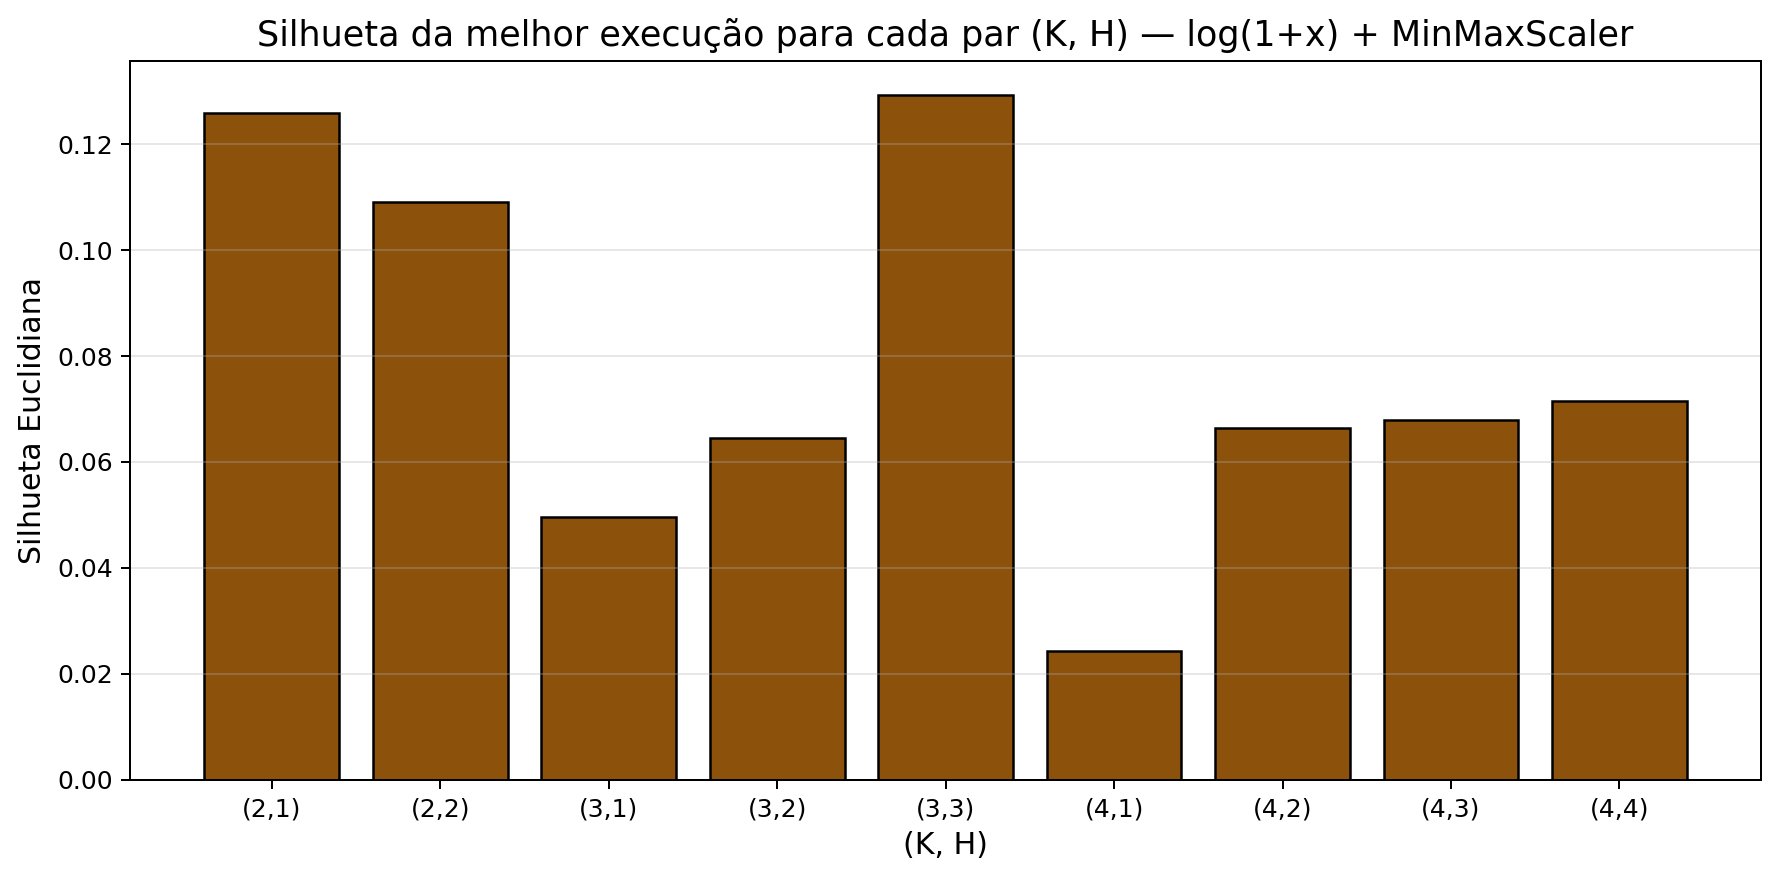
\includegraphics[width=\linewidth,height=2.9cm,keepaspectratio]{../../questao1/resultados/log_minmax/silhouette_KH.png}
\vspace{1mm}
\begin{notabox}\centering\small\textbf{$(K^*,H^*)=(3,3)$} \quad Sil. $=0,1292$ \quad ARI $=0,3911$\end{notabox}
\end{columns}
\vspace{2mm}
\begin{alertabox}\scriptsize \textbf{Critério:} 100 reinícios por par; menor $W$, depois maior Silhueta dentro da representação. \textbf{Ressalva:} o ARI foi consultado depois para escolher entre representações; a decisão não foi totalmente cega aos rótulos.\end{alertabox}
\end{frame}

% 08 - 00:40 - resultado q1
\begin{frame}[t]{Q1 | Que estrutura o Double K-means encontrou?}
\begin{columns}[T,onlytextwidth]
\column{.55\textwidth}
\small \textbf{Clusters de e-mails × classes originais}
\vspace{1.5mm}
\footnotesize
\renewcommand{\arraystretch}{1.45}
\begin{tabular}{lrrr}
\toprule
Grupo & Não-spam & Spam & Total\\
\midrule
\textbf{Cluster 0} & 2.218 & 401 & 2.619\\
\textbf{Cluster 1} & 265 & 0 & 265\\
\textbf{Cluster 2} & 305 & 1.412 & 1.717\\
\bottomrule
\end{tabular}
\vspace{2.5mm}
\begin{notabox}\small\textbf{ARI = 0,3911}: correspondência parcial, não reprodução perfeita das classes conhecidas.\end{notabox}
\column{.43\textwidth}
\begin{simplebox}
\textbf{Como ler a solução}\par\vspace{1mm}
\small
\begin{itemize}\setlength\itemsep{1.5mm}
\item \textbf{3 grupos de objetos} ($K=3$).
\item \textbf{3 blocos de atributos} ($H=3$), com protótipos em $G$.
\item Melhor execução convergiu em \textbf{14 iterações}.
\end{itemize}
\end{simplebox}
\end{columns}
\vspace{2mm}
\begin{alertabox}\small \textbf{Consequência:} esses três grupos passaram a ser o segundo alvo supervisionado da Questão 2 --- mantendo os mesmos 57 preditores brutos.\end{alertabox}
\end{frame}

% 09 - 00:45 - desenho q2
\begin{frame}[t]{Decisão 3 | Nunca usar o teste para ajustar o modelo}
\vspace{1mm}
\begin{columns}[T,onlytextwidth]
\column{.58\textwidth}
\begin{tikzpicture}[>=Stealth,node distance=4mm,
box/.style={draw=cinazul!35,fill=azulclaro!23,rounded corners=2pt,text width=6.2cm,align=center,minimum height=1.04cm,font=\small}]
\node[box] (a) {\textbf{30 repetições × 10 folds estratificados}\\Separar 9 folds de treino e 1 de teste};
\node[box,below=of a] (b) {\textbf{CV interna de 5 folds}\\Selecionar hiperparâmetros por F1 macro};
\node[box,below=of b] (c) {\textbf{Reajustar nos 9 folds}\\Avaliar uma única vez no fold externo};
\draw[->,thick,cinazul] (a)--(b);
\draw[->,thick,cinazul] (b)--(c);
\end{tikzpicture}
\column{.39\textwidth}
\begin{simplebox}
\small\textbf{Cuidados efetivos}\par\vspace{1mm}
\begin{itemize}\setlength\itemsep{1.4mm}
\item Mesmos folds para os 5 modelos.
\item \texttt{log1p + MinMax} ajustado \emph{dentro} do treino.
\item Métricas macro para não ocultar a classe de 265 casos.
\end{itemize}
\end{simplebox}
\end{columns}
\vspace{2mm}
\begin{notabox}\scriptsize O alvo de 3 clusters foi construído previamente sobre a base inteira: sua avaliação supervisionada mede \textbf{reprodução de uma partição fixa}, não generalização externa de novos clusters.\end{notabox}
\end{frame}

% 10 - 00:40 - modelagem
\begin{frame}[t]{Decisão 4 | Comparar hipóteses diferentes, com ajuste justo}
\vspace{1mm}
\footnotesize
\renewcommand{\arraystretch}{1.20}
\setlength{\tabcolsep}{4pt}
\begin{tabular}{p{2.3cm}p{5.2cm}p{3.3cm}}
\toprule
\textbf{Classificador} & \textbf{Estratégia que testamos} & \textbf{Ajuste interno}\\
\midrule
Gaussiano multivariado & Densidade por classe; regularizar a covariância para estabilidade. & intensidade $\lambda$\\
Bayes k-NN & Decidir pela proporção de classes na vizinhança. & $k$ + 3 distâncias\\
Bayes Parzen & Estimar densidade com kernels gaussianos produto. & largura $h$\\
Regressão Logística & Fronteiras lineares com regularização $L_2$. & $C$ + pesos das classes\\
Voto Majoritário & Combinar os quatro anteriores; desempate pela priori do treino. & sem grade adicional\\
\bottomrule
\end{tabular}
\vspace{3mm}
\begin{notabox}\small \textbf{Por que assim?} A comparação não se limitou a cinco nomes: ela testou diferentes hipóteses de separação com \textbf{o mesmo protocolo e os mesmos índices de avaliação}.\end{notabox}
\end{frame}

% 11 - 00:50 - resultados principais
\begin{frame}[t]{O melhor método depende do alvo a prever}
\small \textbf{F1 macro médio} nas 30 repetições de 10 folds (barras: 0,75--1,00; maior é melhor).
\vspace{2mm}
\begin{columns}[T,onlytextwidth]
\column{.49\textwidth}
\begin{simplebox}
\textbf{Classes originais (2)}\par\vspace{1mm}
\scorebar{Gaussiano}{0.8471}{0,8471}{cinazul}
\scorebar{k-NN}{0.9290}{0,9290}{cinazul}
\scorebar{Parzen}{0.9394}{0,9394}{ciano}
\scorebar{Logística}{0.9355}{0,9355}{cinazul}
\scorebar{\textbf{Voto}}{0.9397}{\textbf{0,9397}}{verdeescuro}
\end{simplebox}
\column{.49\textwidth}
\begin{simplebox}
\textbf{Clusters descobertos (3)}\par\vspace{1mm}
\scorebar{Gaussiano}{0.7976}{0,7976}{cinazul}
\scorebar{k-NN}{0.9114}{0,9114}{cinazul}
\scorebar{Parzen}{0.9224}{0,9224}{cinazul}
\scorebar{\textbf{Logística}}{0.9827}{\textbf{0,9827}}{verdeescuro}
\scorebar{Voto}{0.9347}{0,9347}{cinazul}
\end{simplebox}
\end{columns}
\vspace{1mm}
\begin{notabox}\small\textbf{Original:} Voto 0,9397 $\approx$ Parzen 0,9394 (erro: 5,71\% e 5,75\%). \textbf{Clusters:} Logística 0,9827 (erro: 0,95\%). São tarefas diferentes; os F1 não devem ser comparados entre alvos como se fossem a mesma dificuldade.\end{notabox}
\end{frame}

% 12 - 00:40 - estatistica
\begin{frame}[t]{Decisão 5 | Interpretar diferenças, não apenas ordenar médias}
\vspace{1mm}
\begin{columns}[T,onlytextwidth]
\column{.48\textwidth}
\begin{simplebox}
\small\textbf{Friedman, nas quatro métricas}\par\vspace{1mm}
\small Em \textbf{8 de 8 comparações} (2 alvos × 4 métricas), houve evidência global de diferenças entre os 5 modelos ($p<10^{-19}$).
\end{simplebox}
\vspace{2mm}
\begin{notabox}
\small \textbf{Nemenyi, F1 original}\par
\footnotesize Voto × Parzen: $p=0,9883$. Diferença não detectada.
\end{notabox}
\column{.48\textwidth}
\begin{simplebox}
\small\textbf{Nemenyi, F1 dos clusters}\par\vspace{1mm}
\footnotesize Logística × Voto: $p=0,1024$. Diferença não detectada, apesar do maior F1 pontual da Logística.
\end{simplebox}
\vspace{2mm}
\begin{alertabox}
\small\textbf{Cautela:} os ICs e os testes são descritivos/exploratórios, pois as 30 repetições reutilizam as mesmas 4.601 instâncias.
\end{alertabox}
\end{columns}
\vspace{2mm}
\small\color{cinzaescuro}Foram avaliados erro, precisão, cobertura e F1 macro, com estimativas e ICs de 95\%; tabelas detalhadas constam do relatório.
\end{frame}

% 13 - 00:40 - curvas
\begin{frame}[t]{Curvas de aprendizagem | O que muda com mais dados?}
\vspace{1mm}
\begin{columns}[T,onlytextwidth]
\column{.49\textwidth}
\centering\small\textbf{Rótulos originais: F1 de teste}\\[1mm]
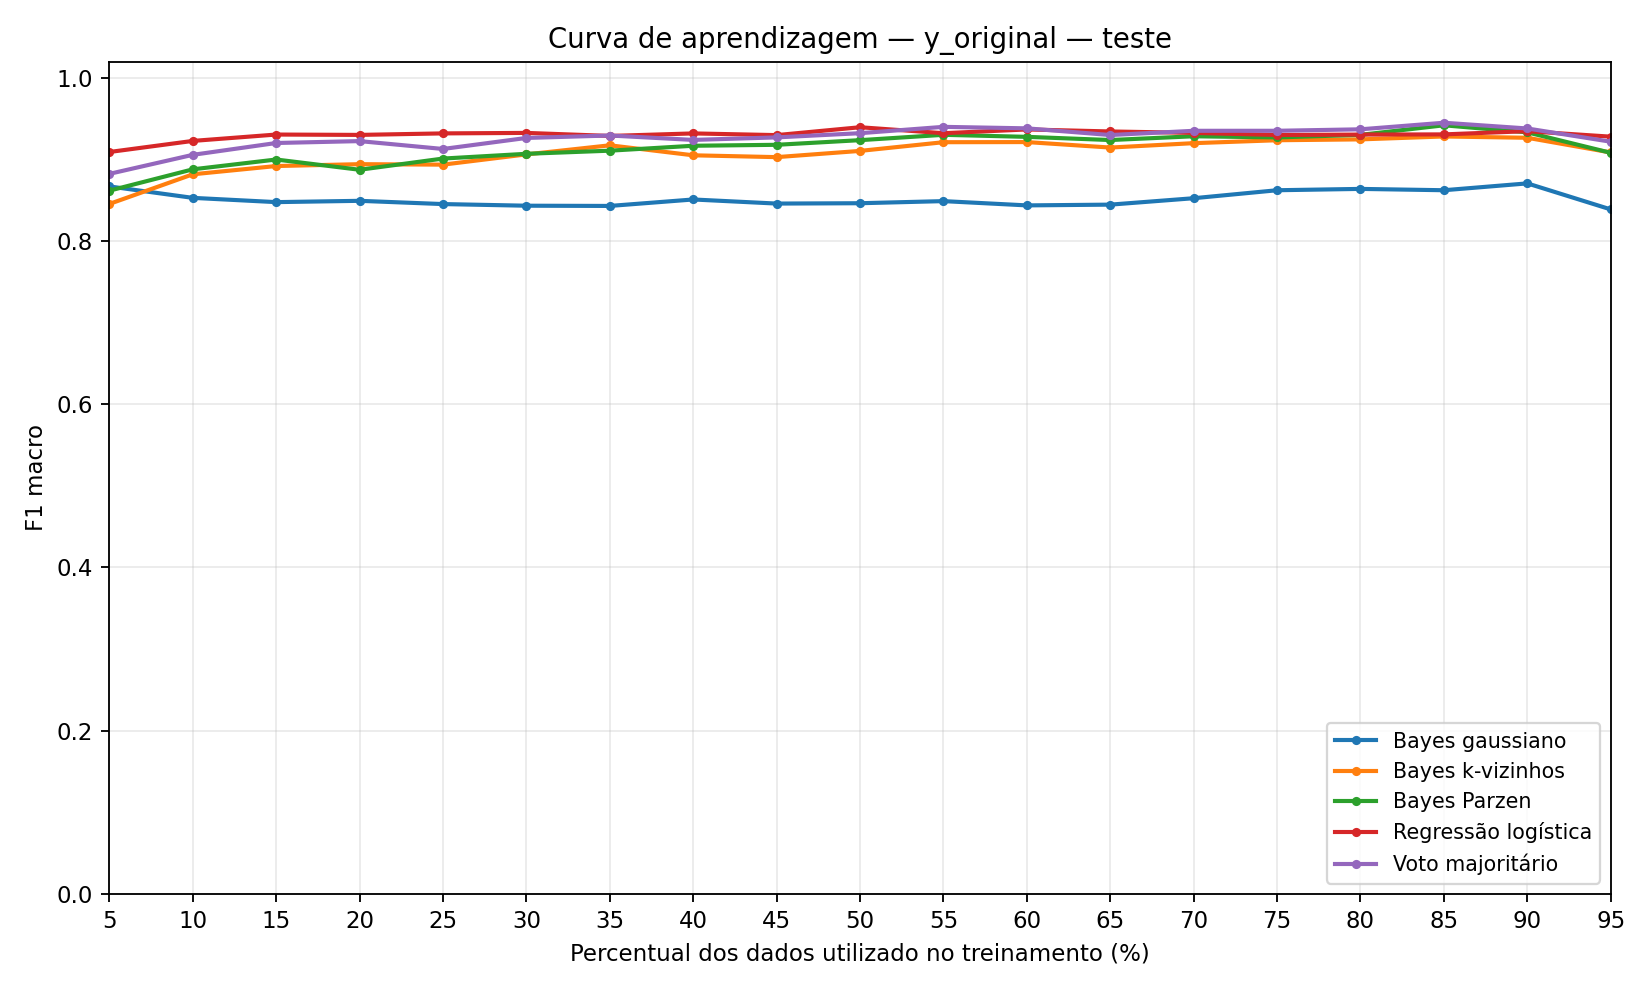
\includegraphics[width=\linewidth,height=3.85cm,keepaspectratio]{../../questao2/resultados/curvas_aprendizagem/graficos/y_original_f1_teste.png}
\column{.49\textwidth}
\centering\small\textbf{Clusters: F1 de teste}\\[1mm]
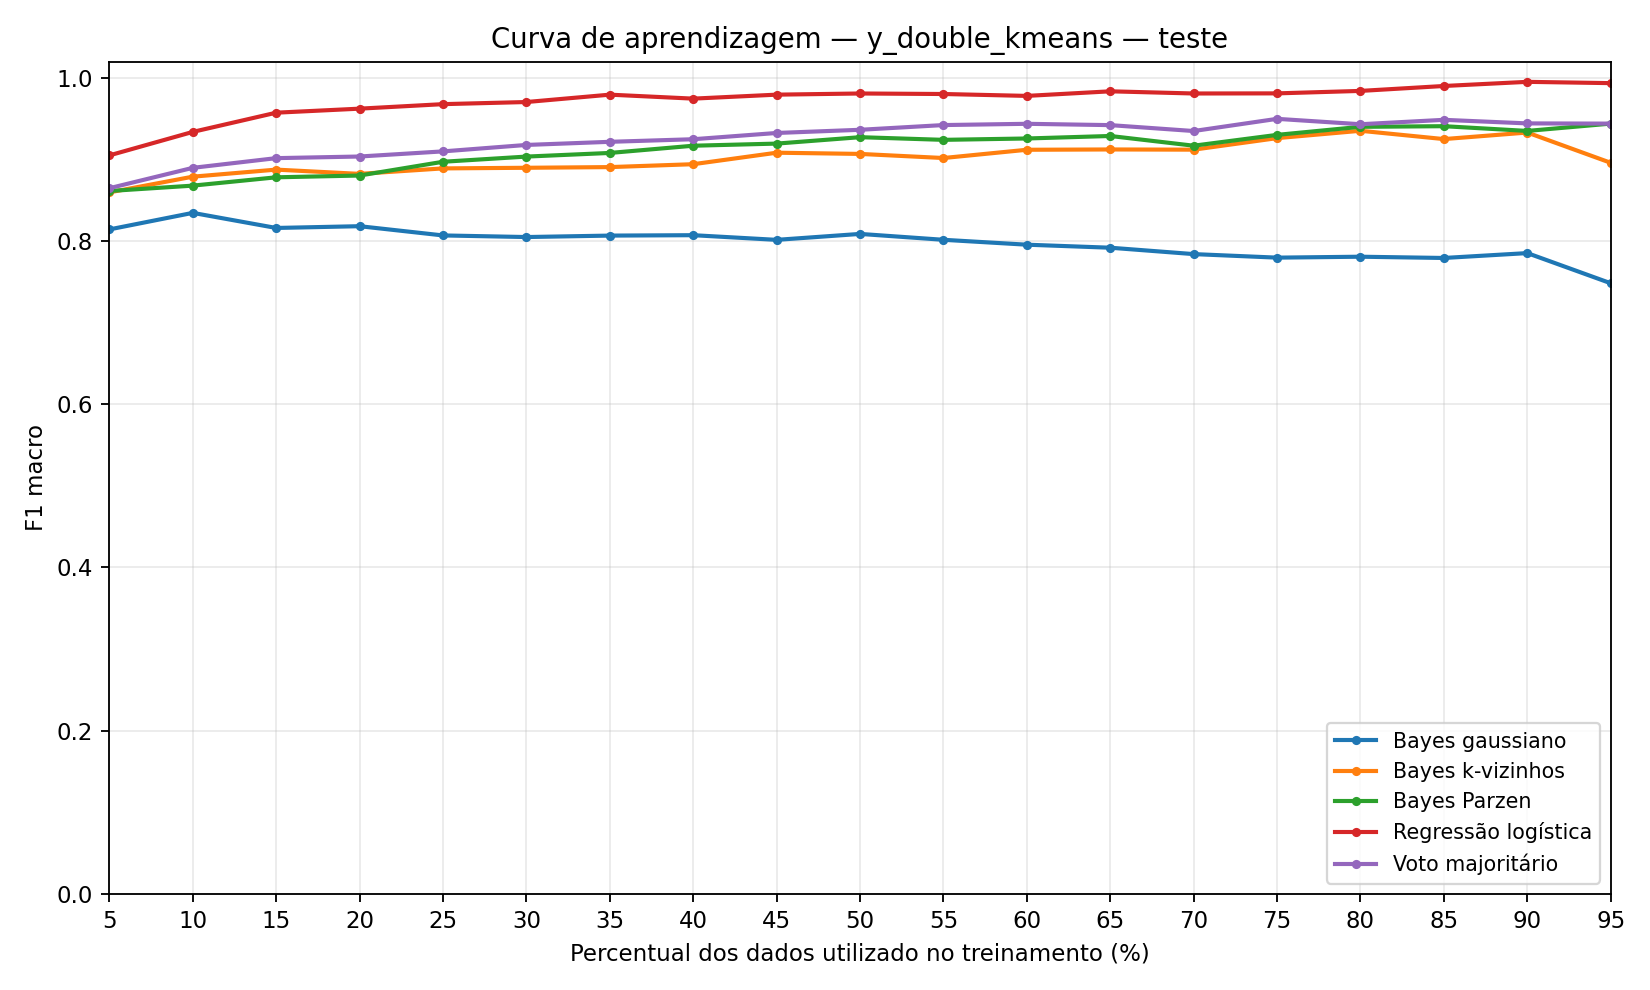
\includegraphics[width=\linewidth,height=3.85cm,keepaspectratio]{../../questao2/resultados/curvas_aprendizagem/graficos/y_double_kmeans_f1_teste.png}
\end{columns}
\vspace{1mm}
\begin{notabox}\scriptsize Treinamento de 5\% a 95\%, em passos de 5\%. As curvas completas de \textbf{treino e teste} estão no relatório. Com clusters, a Logística alcança F1 de teste 0,9050 (5\%) e 0,9936 (95\%); os extremos têm testes menores.\end{notabox}
\end{frame}

% 15 - 00:25 - conclusoes
\begin{frame}[t]{Três conclusões que defendemos}
\vspace{1mm}
\begin{simplebox}
\textbf{1. A representação definiu o agrupamento.}\par
\small Uma Silhueta alta ocultou um microcluster. Com \texttt{log1p + MinMax}, obtivemos $K^*=H^*=3$ e ARI 0,3911, após escolher a representação também com consulta ao ARI.
\end{simplebox}
\vspace{1mm}
\begin{simplebox}
\textbf{2. A comparação exigiu disciplina experimental.}\par
\small Mesmos folds, CV interna e pré-processamento restrito ao treino evitaram usar os folds de teste no ajuste.
\end{simplebox}
\vspace{1mm}
\begin{simplebox}
\textbf{3. O melhor F1 depende do alvo.}\par
\small Voto/Parzen nas classes originais; Logística na reprodução dos clusters. Testes exploratórios e natureza transdutiva exigem cautela.
\end{simplebox}
\end{frame}

% 16 - Encerramento e referencias
\begin{frame}[t]{Obrigado!}
\begin{notabox}[top=1.2mm,bottom=1.2mm,before skip=1mm,after skip=1.5mm]
\centering
{\normalsize\bfseries\color{cinazul}Perguntas?}\par\vspace{0.8mm}
\scriptsize \textbf{Repositório:} \texttt{https://github.com/fal6-cin/projetoAM20262Q1}\par\vspace{0.6mm}
\scriptsize \textbf{Contato:} Douglas Araújo Silva (\texttt{das7@cin.ufpe.br}), Felipe Araújo de Lima (\texttt{fal6@cin.ufpe.br}), Letícia De Albuquerque S. Leitão (\texttt{lasl@cin.ufpe.br})
\end{notabox}
\begin{simplebox}[top=1.2mm,bottom=1.2mm,before skip=1mm,after skip=0mm]
\footnotesize\textbf{Referências principais}\par\vspace{0.6mm}
\scriptsize
\begin{enumerate}\setlength\itemsep{0.6mm}
\item \textbf{Carvalho, F. A. T. de (2026).} \emph{Notas de Aula e Especificação do Projeto — IN1102}, CIn/UFPE.
\item \textbf{Hopkins, M. et al. (1999).} \emph{Spambase Dataset}. HP Labs / UCI ML Repository (\texttt{archive.ics.uci.edu/dataset/94/spambase}).
\item \textbf{Kittler, J., Hatef, M., Duin, R. P. W., \& Matas, J. (1998).} On combining classifiers. Vol. 20, no. 3, pp. 226--239, doi: \texttt{10.1109/34.667881}.
\item \textbf{Dem\v{s}ar, J. (2006).} Statistical Comparisons of Classifiers over Multiple Data Sets. \emph{JMLR}, 7, 1--30.
\end{enumerate}
\end{simplebox}
\end{frame}

\end{document}
